% Created 2019-11-09 Sat 23:07
\documentclass[11pt]{article}
\usepackage[utf8]{inputenc}
\usepackage[T1]{fontenc}
\usepackage{fixltx2e}
\usepackage{graphicx}
\usepackage{longtable}
\usepackage{float}
\usepackage{wrapfig}
\usepackage{rotating}
\usepackage[normalem]{ulem}
\usepackage{amsmath}
\usepackage{textcomp}
\usepackage{marvosym}
\usepackage{wasysym}
\usepackage{amssymb}
\usepackage{hyperref}
\tolerance=1000
\usepackage{palatino}
\usepackage[top=1in,bottom=1.25in,left=1.25in,right=1.25in]{geometry}
\usepackage{setspace}
\setcounter{secnumdepth}{1}
\author{Praveen Kumar R}
\date{\today}
\title{Image Processing}
\hypersetup{
  pdfkeywords={},
  pdfsubject={},
  pdfcreator={Emacs 25.2.2 (Org mode 8.2.10)}}
\begin{document}

\maketitle
\section{Computer Vision}
\label{sec-1}
Computer Vision is the branch of Computer science that lays protocol for computer and    
other machines to how to see the ouside world. Object detection, Rendering Segmented mask,    
Pattern recognition, Image transfromation and preprocessring,etc., are some of the major   
goals of this branch of study. Recently CV has evolved to visualise more mathematically    
complicated concepts like fuzzy logic, laplace transformation, Abstract Algebra, etc.,    
thus giving these concepts a better scope of understanding.

\section{What is an Image?}
\label{sec-2}
An image in its fundementel level is conceptualised as a collection of meaningful pixels.   
On the basis of how an image is constructed from it atomic stage, images can be classified   
into many categories
\begin{itemize}
\item RGB images
\item HSV images
\item CMYK images
\item HWB images
\item HEX images
\end{itemize}
etc,.
Each of these categories differ in syntax of how the color of each pixel is represented. A same image   
represented in these different formats will differ in quality and color. This is because some   
formats dosent give the liberty to choose many colors. RGB format is generally adapted   
for any kind of image processing technique.   

\section{RGB Image}
\label{sec-3}
Every pixel in a RGB image is defined by 3 values Red, Green, and Blue. Each of these values   
uses 8 bit standard(IEEE) representation. 7 bits to represent value and the most significant bit   
to represent sign. Thus each of the values for R,G and B will run from 0 t0 255. As the value of   
ceratain channel reaches 0 the brightness of the color imparted by that channel tend to become low, meaning the channel will become deeper in color and eventually become black.
Similarly as the value of a certain channel approches to 255 the color imparted by that channel    becomes
more brighter. From the above statements one may arrive at the following hypothesis,   
\begin{itemize}
\item (0,0,0) : will be black color
\item (255,255,255): will be white color
\item (255,0,0) : will be bright red color
\item (0,255,0) : will be bright green color
\item (0,0,255) : will be bright blue colors
\end{itemize}
the representation is based on the assumption that pixel representation is in RGB format.   
By fundemental principle of counting the number of different colors that can be formed is   
256 x 256 x 256 = 16,777,216    
\begin{figure}[htb]
\centering
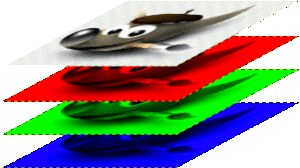
\includegraphics[width=250px]{./rgb.png}
\caption{\label{fig1}RGB image - The top layer shown is the actual image you see. But it actually represented using 3 different channels}
\end{figure}

Mathematically a 3 channel RGB image is modeled as a 4 dimensinol matrix. The inner most dimension   
will provide information about the pixel value. The next dimension will be an vector of these pixels forming   
rows of the image channel matrix. These rows combine in next dimension vertically to form a channel. Three such   
channels will combine to form a RGB image. In case of Grayscale image there will be only one channel, and each pixel   
is defined by one single value ranging from 0 to 255(extremes inclusive).  

\section{Installation}
\label{sec-4}
OpenCV is a open source community the keep constantly updating its libraries  
based on input from programmers all around the world. OpenCV is available in two  
different distribution Python and C++. Though the functionality of both the distribution  
are maintained to be the same, the syntax and the parameters differ in each of these language  
distributions. In this guide you will be able to install the python distribution of opencv.  
The commands in this installation steps were tried and tested in Ubuntu 18.04.  

\section{Pre-requisite}
\label{sec-5}
It is recommended that the programmer uses a linux or unix based operating system like  
Ubuntu, Kali, or MacOS. Standard distribution for python comes pre installed with  
these opearting system. To check the version of python run the following command.  
\begin{verbatim}
$ python --version
\end{verbatim}
If python package is not found in your system install the package by running the  
following commands.  
\begin{verbatim}
$ sudo add-apt-repository ppa:jonathonf/python-3.6
$ sudo apt-get update
$ sudo apt-get install python3.6
\end{verbatim}
\section{Installation Steps}
\label{sec-6}
To install addtional libraries for python you need either one of the installation tools  
\begin{itemize}
\item pip
\item pip3 (recommended for python3)
\item conda
\end{itemize}
\subsection*{pip}
\label{sec-6-1}
To install pip use the following command.

\begin{verbatim}
sudo apt-get install python3-pip
\end{verbatim}
\subsection*{pip3}
\label{sec-6-2}
You can upgrade your pip to pip3 by running the following command.
\begin{verbatim}
sudo -H pip3 install --upgrade pip
\end{verbatim}
\subsection*{conda}
\label{sec-6-3}
To install conda download the conda bash .sh file from [[\url{http://repo.anaconda.com/archive/Anaconda3-2019.03-Linux-x86_64.sh}]]
Once the download is complete go to the directory where the extracted .sh file is present  
and run the following command.  
\begin{verbatim}
bash Anaconda3-2019.03-Linux-x86_64.sh
\end{verbatim}
\textbf{\textbf{NOTE:}} The bash command will vary with name of the .sh script installed. So remember  
 to give the correct file name in the command. \newline 

I would recommend to install all these tools because some of the libraries are easily  
installed using each of these tools.  

\subsection*{Dependency packages}
\label{sec-6-4}
You can download this \href{https://github.com/pbcpraveen/I-Cell/blob/master/Introduction\%20to\%20Images/Installation/tensorlfow.sh}{bashscripts} that contains all commands for the installation.
You can directly execute this file after changing the permissions of the file.
The program requires the following packages for execution  
\begin{verbatim}
opencv
numpy
pandas
theano
tensorflow
keras
pillow
\end{verbatim}
Before installing any of these libraries I would recommend you to create a new environment
in your your conda to avoid libraries version clashes. To create a new environment run the following 
command in your terminal.
\begin{verbatim}
conda create --name myenv
\end{verbatim}
By running the above command you will create a new environment called 'myenv'. In most of the terminal
the command prompt message is preceeded with the environment where you are currently in. The default conda 
environment is called 'base' to move to another environment run the following command.
\begin{verbatim}
conda activate myenv
\end{verbatim}
or 
\begin{verbatim}
source activate myenv
\end{verbatim}
Once you land your newly created environment you are ready to install the packages. Run the following commands to install the
packages mentioned above. Using conda is useful because conda will take care of the libraries verions to be installed.  
\begin{verbatim}
$ conda install -c anaconda numpy 
$ conda install -c anaconda pandas 
$ conda install -c conda-forge opencv 
$ conda install -c conda-forge theano 
$ conda install -c conda-forge tensorflow 
$ conda install -c conda-forge keras
$ conda install -c anaconda pillow
$ python3 -m pip install ipykernel
$ python3 -m ipykernel install --user
\end{verbatim}


\textbf{\textbf{Note:}} If you are willing to install the tensorflow and keras for GPU, do it  
only if you have good Graphical processing unit in you machine, because it is  
tedious process. For GPU installation follow the instruction in the [[\url{https://www.tensorflow.org/install/gpu}]] 
\textbf{\textbf{GOOD LUCK}}
\newpage

\section{Introduction to OpenCV python3}
\label{sec-7}
\subsection*{Importing libraries}
\label{sec-7-1}
To start with import the necessary libraries for the for the programmer  
\begin{verbatim}
import cv2
import numpy
\end{verbatim}
if any of the above import fails it means that you made mistake in you installation  
process. Then go back to the previous section and reinstall all the libraries after  
removing them.  
\subsection*{Reading images}
\label{sec-7-2}
To read a image and store it in a variable use the imread function.  
\begin{verbatim}
img = cv2.imread('sampleImage.jpg')
\end{verbatim}
the above line will read a image named `sampleImage.jpg` from the present working directory.  
The image read is by default in BGR format , to read the image in gray scale replace the above  
line with  
\begin{verbatim}
img = cv2.imread('sampleImage.jpg',0)
\end{verbatim}
The image read is a numpy array. Thus you can create you own image by creating an numpy array  
with a element with 8 bit representation  
\begin{verbatim}
img = np.ones((300,400,3),dtype = np.uint8)*255
\end{verbatim}
the above line will create a 3 channel image with height 300 and 400 pixels fill all pixel values  
to (255,255,255), meaning the image will be a white image.  
\subsection*{Displaying images}
\label{sec-7-3}

To display an image cv2 provides a function called `imshow`  
\begin{verbatim}
cv2.imshow('window_name',img)
\end{verbatim}
If you run your code now your program might probably collapse and the window  
will stop responding. This is because once the imshow fuction is called the program  
will create a thread (child thread) to display the image but as soon as the child thread  
is created the parent process terminates leaving the child thread in orphan state.  
Thus the window will not repond to any clicks. So to avoid it always use the imshow function  
with a function called `waitKey()` to make the parent process to wait till the child terminates  
and close all the windows before you exit the program.  
\begin{verbatim}
cv2.imshow('window_name',img)
cv2.waitKey(0)
cv2.destroyAllWindows()
\end{verbatim}
\textbf{\textbf{NOTE:}} `cv2.waitKey(0)` will make the program to halt and wait until a keyboard stroke  
is recieved. In case of video where the frame are continuously read, waiting for key board stroke will  
not be a efficient job to do, so we we give waitKey(1) where the program don't halt but continue executing  
and scans for keyboard stroke in interval of 1 sec.  
\newpage
So a Simple program will look like  
\begin{verbatim}
import cv2
import numpy as np

img = cv2.imread('sampleImage.jpg')

cv2.imshow('Image',img)
cv2.waitKey(0)
cv2.destroyAllWindows()
\end{verbatim}

So to display a live video use this program  
\begin{verbatim}
import cv2
import numpy as np

cap = cv2.VideoCapture(0)
while True:
   ret,frame = cap.read()
   cv2.imshow('video',frame)
   if(cv2.waitKey(1)==13):
      break
cap.release()
cv2.destroyAllWindows()
\end{verbatim}
\begin{figure}[htb]
\centering
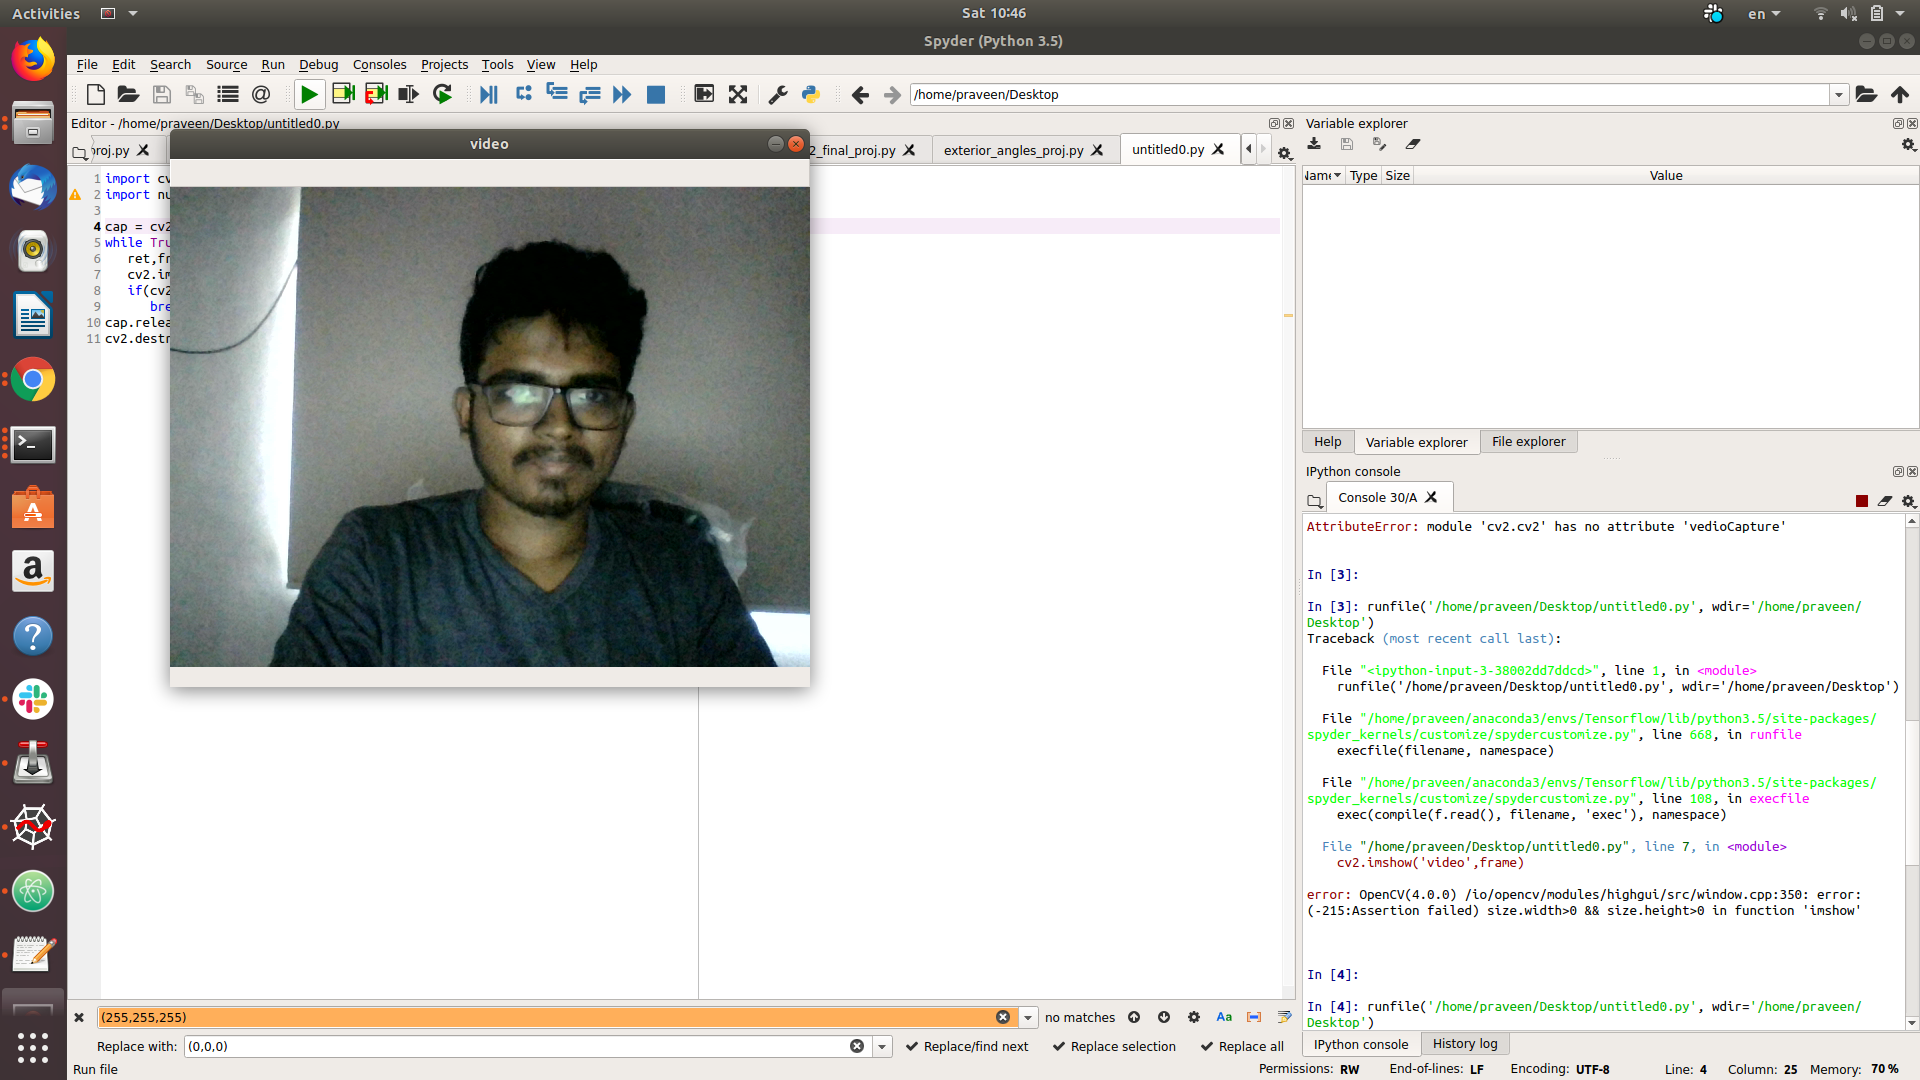
\includegraphics[width=250px]{./videoDemo2.png}
\caption{\label{fig1}Output}
\end{figure}
% Emacs 25.2.2 (Org mode 8.2.10)
\end{document}
